\begin{figure}
    \centering
    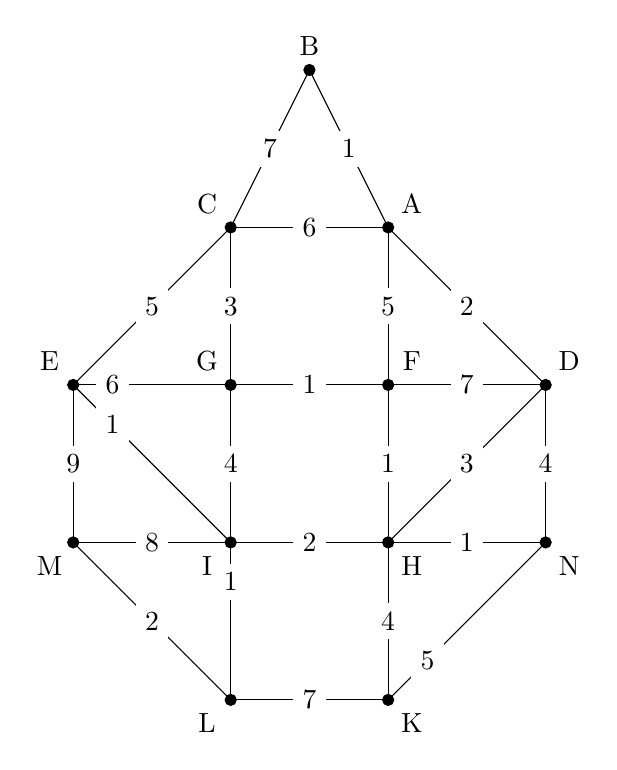
\begin{tikzpicture}

%% vertices
\draw[fill=black] (4,6) circle (2pt);   %% a
\draw[fill=black] (3,8) circle (2pt);   %% b
\draw[fill=black] (2,6) circle (2pt);   %% c
\draw[fill=black] (6,4) circle (2pt);   %% d
\draw[fill=black] (0,4) circle (2pt);   %% e
\draw[fill=black] (4,4) circle (2pt);   %% f
\draw[fill=black] (2,4) circle (2pt);   %% g
\draw[fill=black] (4,2) circle (2pt);   %% h
\draw[fill=black] (2,2) circle (2pt);   %% i
\draw[fill=black] (4,0) circle (2pt);   %% k
\draw[fill=black] (2,0) circle (2pt);   %% l
\draw[fill=black] (0,2) circle (2pt);   %% m
\draw[fill=black] (6,2) circle (2pt);   %% n


%% vertex labels
\node at (4.3,6.3) {A};
\node at (3,8.3) {B};
\node at (1.7,6.3) {C};
\node at (6.3,4.3) {D};
\node at (-0.3,4.3) {E};
\node at (4.3,4.3) {F};
\node at (1.7,4.3) {G};
\node at (4.3,1.7) {H};
\node at (1.7,1.7) {I};
\node at (4.3,-0.3) {K};
\node at (1.7,-0.3) {L};
\node at (-0.3,1.7) {M};
\node at (6.3,1.7) {N};

%%% edges
\draw (4,6) -- (3,8) node [midway, fill=white] {1};     %% ab
\draw (4,4) -- (2,4) node [midway, fill=white] {1};     %% fg
\draw (4,4) -- (4,2) node [midway, fill=white] {1};     %% fh
\draw (4,2) -- (6,2) node [midway, fill=white] {1};     %% hn
\draw (0,4) -- (2,2) node [near start, fill=white] {1}; %% ei
\draw (2,2) -- (2,0) node [near start, fill=white] {1}; %% il
\draw (4,6) -- (6,4) node [midway, fill=white] {2};     %% ad
\draw (4,2) -- (2,2) node [midway, fill=white] {2};     %% hi
\draw (2,0) -- (0,2) node [midway, fill=white] {2};     %% lm
\draw (6,4) -- (4,2) node [midway, fill=white] {3};     %% dh
\draw (2,6) -- (2,4) node [midway, fill=white] {3};     %% cg
\draw (4,2) -- (4,0) node [midway, fill=white] {4};     %% hk
\draw (6,4) -- (6,2) node [midway, fill=white] {4};     %% dn
\draw (2,4) -- (2,2) node [midway, fill=white] {4};     %% gi
\draw (2,6) -- (0,4) node [midway, fill=white] {5};     %% ce
\draw (4,6) -- (4,4) node [midway, fill=white] {5};     %% af
\draw (4,0) -- (6,2) node [near start, fill=white] {5}; %% kn
\draw (0,4) -- (2,4) node [near start, fill=white] {6}; %% eg
\draw (4,6) -- (2,6) node [midway, fill=white] {6};     %% ac
\draw (3,8) -- (2,6) node [midway, fill=white] {7};     %% bc
\draw (4,0) -- (2,0) node [midway, fill=white] {7};     %% kl
\draw (6,4) -- (4,4) node [midway, fill=white] {7};     %% df
\draw (2,2) -- (0,2) node [midway, fill=white] {8};     %% im
\draw (0,4) -- (0,2) node [midway, fill=white] {9};     %% em
    \end{tikzpicture}
    \label{question3-a}
    \caption{Graph in question 3}
\end{figure}